\documentclass[11pt]{article}
%prepared in AMSLaTeX, under LaTeX2e
\addtolength{\oddsidemargin}{-.75in} 
\addtolength{\evensidemargin}{-.75in}
\addtolength{\topmargin}{-.6in}
\addtolength{\textwidth}{1.4in}
\addtolength{\textheight}{1.3in}

\renewcommand{\baselinestretch}{1.075}

\usepackage{verbatim,fancyvrb}

\usepackage{palatino,amsmath,amssymb,amsthm}

\usepackage{tikz}
\usetikzlibrary{arrows.meta}

\newtheorem*{thm}{Theorem}
\newtheorem*{defn}{Definition}
\newtheorem*{example}{Example}
\newtheorem*{problem}{Problem}
\newtheorem*{remark}{Remark}

\newcommand{\mtt}{\texttt}
\usepackage{alltt,xspace}

%\usepackage[final]{graphicx}

\usepackage[pdftex, colorlinks=true, plainpages=false, linkcolor=blue, citecolor=red, urlcolor=blue]{hyperref}

% macros
\newcommand{\bc}{\mathbf{c}}
\newcommand{\br}{\mathbf{r}}
\newcommand{\bv}{\mathbf{v}}
\newcommand{\bx}{\mathbf{x}}
\newcommand{\by}{\mathbf{y}}

\newcommand{\CC}{\mathbb{C}}
\newcommand{\RR}{\mathbb{R}}
\newcommand{\ZZ}{\mathbb{Z}}

\newcommand{\eps}{\epsilon}
\newcommand{\grad}{\nabla}
\newcommand{\lam}{\lambda}
\newcommand{\lap}{\triangle}

\newcommand{\ip}[2]{\ensuremath{\left<#1,#2\right>}}

%\renewcommand{\det}{\operatorname{det}}
\newcommand{\onull}{\operatorname{null}}
\newcommand{\rank}{\operatorname{rank}}
\newcommand{\range}{\operatorname{range}}

\newcommand{\prob}[1]{\bigskip\noindent\textbf{#1.}\quad }
\newcommand{\exer}[2]{\prob{Exercise #2 in Lecture #1}}

\newcommand{\pts}[1]{(\emph{#1 pts}) }
\newcommand{\epart}[1]{\medskip\noindent\textbf{(#1)}\quad }
\newcommand{\ppart}[1]{\,\textbf{(#1)}\quad }

\newcommand{\Julia}{\textsc{Julia}\xspace}
\newcommand{\Matlab}{\textsc{Matlab}\xspace}
\newcommand{\Octave}{\textsc{Octave}\xspace}
\newcommand{\Python}{\textsc{Python}\xspace}

\DefineVerbatimEnvironment{mVerb}{Verbatim}{numbersep=2mm,
frame=lines,framerule=0.1mm,framesep=2mm,xleftmargin=4mm,fontsize=\footnotesize}

\newcommand{\ema}{\emach}
\newcommand{\emach}{\eps_{\!_{\text{m}}}}

\title{POPDIP: \\ a POsitive-variables Primal-Dual Interior Point method}
\author{Ed Bueler}
\date{\today}

\begin{document}
\maketitle

\begin{abstract}
The algorithm documented here is a version of a Newton-type primal-dual interior point algorithm in \cite{GrivaNashSofer2009}, namely Algorithm 16.1 in section 16.7.  The version here minimizes a smooth nonlinear function subject to the simple constraints that all the variables are nonnegative.  That is, it is a specialized algorithm for nonnegativity constraints; it is not suitable for general inequality constraints.

These short notes are not research!  This algorithm is simply a special case of a well-known algorithm.  Furthermore ``POPDIP'' is just a name I made up; it is not in common use!  However, this class of algorithms is new to me so I am documenting it fully.
\end{abstract}

\thispagestyle{empty}

\bigskip
\subsection*{Introduction}

Consider a nonlinear optimization problem with nonnegativity (informally: positivity) constraints on the variables:
\begin{equation}
\begin{matrix}
\text{minimize} \qquad & f(x) \\
\text{subject to} \qquad & x \ge 0
\end{matrix} \label{minproblem}
\end{equation}
As usual, ``$x\ge 0$'' means that each entry of $x\in\RR^n$ is nonnegative.  The feasible set for \eqref{minproblem} is the convex and closed set $S = \{x\in \RR^n\,:\,x\ge 0\}$ with interior $S^\circ = \{x\in \RR^n\,:\,x > 0\}$.

Here $f:\RR^n \to\RR^n$ is a continuous and smooth function.  In fact this algorithm only assumes $f$ is defined and smooth on $S^\circ$, but in practice, so as to have a chance of good performance, $f$ should be well-behaved near the boundary of $S$.

One can start the derivation by considering a logarithmic barrier function.  Let $\mu>0$.  If $x\in S^\circ$ then the following function is well-defined and finite:
\begin{equation}
\beta_\mu(x) = f(x) - \mu \sum_{i=1}^n \ln x_i \label{barrierfunction}
\end{equation}
Let $\{e_1,\dots,e_n\}$ be the standard basis of $\RR^n$.  The first-order necessary condition for the unconstrained problem of minimizing $\beta_\mu$, namely $\grad \beta_\mu(x)=0$ for $x \in S^\circ$, is
\begin{equation}
\grad f(x) - \mu \sum_{i=1}^n \frac{1}{x_i} e_i = 0 \label{firstorderbarrier}
\end{equation}

Conditions \eqref{firstorderbarrier} can be reformulated by defining additional variables
    $$\lambda_i = \frac{\mu}{x_i}$$
so that $\lambda\in\RR^n$.  Note that $\lambda>0$ if and only if $x>0$ because $\lambda_i x_i = \mu > 0$.  Then \eqref{firstorderbarrier}, plus feasibility for $x$, is precisely equivalent to the following nonlinear system of equations and inequalities:
\begin{align}
x &\ge 0 \label{firstordersystem} \\
\lambda &\ge 0 \notag \\
\grad f(x) - \lambda &= 0 \notag \\
\lambda_i x_i &= \mu, \qquad i=1,\dots,n \notag
\end{align}

The feasible set for $x$ and for $\lambda$ is the same, namely $S \subset \RR^n$.  Because of the last condition in \eqref{firstordersystem}, both $x$ and $\lambda$ are positive and thus in the interior $S^\circ$.  By contrast, for the general primal-dual interior point Algorithm 16.1 \cite[section 16.7]{GrivaNashSofer2009}, the feasible set for the primal variable $x$ is different from the dual feasible set for $\lambda$.  For example, generally the dimension is different.

The third condition in \eqref{firstordersystem} can be written using a Lagrangian function for \eqref{minproblem}, namely
\begin{equation}
\mathcal{L}(x,\lambda) = f(x) - \sum_{i=1}^n \lambda_i x_i,  \label{Lagrangian}
\end{equation}
in which case it states that $\grad_x \mathcal{L}(x,\lambda)=0$.  However, system \eqref{firstordersystem} describes a solution which is different from the KKT conditions for \eqref{minproblem}.  (See Lemma 14.8 and Theorem 14.18 in \cite{GrivaNashSofer2009}.)  Those KKT conditions are the same as system \eqref{firstordersystem} but with the last equation replaced by
\begin{equation}
\lambda_i x_i = 0, \qquad i=1,\dots,n  \label{complementaryslackness}
\end{equation}
That is, complementary slackness applies in the KKT conditions.  System \eqref{firstordersystem} modifies the KKT conditions by connecting the variables through equality with a positive constant ($\lambda_i x_i = \mu$).

Also, the stationary-point conditions for Lagrangian \eqref{Lagrangian}, namely $\grad_x\mathcal{L}(x,\lambda)=0$ and $\grad_\lambda\mathcal{L}(x,\lambda)=0$, do not generally apply because we have nonnegativity constraints on $x$ and \emph{not} equality constraints (which would make the problem trivial).  Of course $x_i=0$ holds when the $i$th constraint is active, but the algorithm here will not keep track of the active set.


\subsection*{Algorithm design}

Algorithm 16.1 \cite{GrivaNashSofer2009} applies to \eqref{minproblem}, and the POPDIP algorithm proposed below is the simplification which uses the fact that $g_i(x)=x_i$.  All such primal-dual interior point algorithms compute approximate solutions to systems like \eqref{firstordersystem} for a sequence $\{\mu_k\}$ going to zero.  In the limit where $\mu=0$, which is never achieved because the algorithm is terminated after a finite number of steps, the solution will solve \eqref{complementaryslackness}.

Each step of the algorithm is a Newton step for the equalities in \eqref{firstordersystem}, namely
\begin{align}
\grad f(x) - \lambda &= 0 \label{equalitysystem} \\
\lambda_i x_i &= \mu_k, \qquad i=1,\dots,n. \notag
\end{align}
The Newton method updates both $x$ and $\lambda$ using the linearization of these equations.  Because of the second equation, these equations are always nonlinear.  Note that if $f$ is quadratic then the first equation is linear.

To describe the Newton step let $x=x_k+\Delta x$ and $\lambda=\lambda_k+\Delta\lambda$.  We assume that the current iterate $(x_k,\lambda_k)$ does not solve \eqref{equalitysystem}.  The unknowns in the Newton step for the search direction $p=(\Delta x,\Delta \lambda)$.  Substituting into \eqref{equalitysystem} and expanding to first order gives
\begin{align}
\grad f(x_k) + \grad^2 f(x_k) \Delta x - \lambda_k - \Delta \lambda &= 0 \label{prenewtonstep} \\
(\lambda_k)_i (x_k)_i + (x_k)_i (\Delta\lambda)_i + (\lambda_k)_i (\Delta x)_i &= \mu_k, \qquad i=1,\dots,n \notag
\end{align}
Rearranging as a linear block system for the search direction, and suppressing the current-iterate subscript, we get the Newton step equations
\begin{equation}
\begin{bmatrix}
\grad^2 f(x) & - I \\
\Lambda & X
\end{bmatrix}
\begin{bmatrix}
\Delta x \\
\Delta \lambda
\end{bmatrix}
=
\begin{bmatrix}
-\grad f(x) + \lambda \\
-\Lambda x + \mu_k e
\end{bmatrix}
 \label{newtonstep}
\end{equation}
Here $I$ is the $n\times n$ identity matrix and the other notation is as follows:
    $$\Lambda = \begin{bmatrix} \lambda_1 & & \\ & \ddots & \\ & & \lambda_n \end{bmatrix}, \qquad X = \begin{bmatrix} x_1 & & \\ & \ddots & \\ & & x_n \end{bmatrix}, \qquad e = \begin{bmatrix} 1 \\ \vdots \\ 1 \end{bmatrix}.$$

Given a solution of \eqref{newtonstep} the update formulas are
\begin{align*}
x_{k+1} &= x_k + \alpha_P \Delta x \\
\lambda_{k+1} &= \lambda_k + \alpha_D \Delta \lambda
\end{align*}
The maximum step sizes $\alpha_P,\alpha_D$ for the primal and dual variables are determined by separate ratio tests to achieve (strict) positivity of $x_{k+1}$ and $\lambda_{k+1}$, respectively.  Because this is a Newton search one uses $\alpha_P=\alpha_D=1$ for the largest allowed step.  Note we are not truly using $p=(\Delta x,\Delta \lambda) \in \RR^{2n}$ as a search direction because of the separate searches for the primal and dual variables.  In fact back-tracking is not needed to maintain feasibility of the primal variables because of the linearity of the constraint functions in \eqref{minproblem}, namely $g_i(x)=x_i$.  As on page 645 for the slack variables, a ratio test on $x$ suffices to keep $x$ feasible.

The optimality test is the same as in Algorithm 16.1 \cite{GrivaNashSofer2009}.  It uses the merit function
\begin{equation}
    \nu(x,\lambda) = \max\{\|\grad f(x)-\lambda\|,\|\Lambda x\|\}  \label{merit}
\end{equation}
where $\|\cdot\|$ denotes the usual $L^2$ norm on $\RR^n$.  Note that once $\mu_k\to 0$ we have $\nu(x_*,\lambda_*) = 0$ for the exact optimum, but when $\mu_k \ne 0$ then the exact solution of \eqref{equalitysystem} does not make $\nu(x,\lambda)$ zero.  In fact $\nu(x_*,\lambda_*) = \sqrt{n}\, \mu_k$ for the exact solution of \eqref{equalitysystem}; if the merit function value $\nu(x_k,\lambda_k)$ is close to $\sqrt{n}\, \mu_k$ then we should decrease $\mu_k$ more rapidly.

Subsection 16.7.2 of \cite{GrivaNashSofer2009} describes how Algorithm 16.1 should be modified so that, by Theorem 16.17, the algorithm will exhibit the local quadratic convergence one would want from a Newton-type algorithm.  Note that quadratic convergence is much harder to achieve in a constrained problem.  This is why I am interested in this algorithm.

First of all the general inequality constraints should be augmented by slack (excess) variables which have simple nonnegativity constraints.  But in our case the constraints are already of that type!  Indeed the general replacement ``$g_i(x)\ge 0$'' by ``$g_i(x) - s_i =0$, $s_i\ge 0$'' is, in our case, the replacement ``$x_i\ge 0$'' by ``$x_i-s_i=0$, $s_i\ge 0$''.  This would be a meaningles renaming of the existing variables, so we need not introduce ``$s_i$'' in our case.

Secondly, Theorem 16.17 uses a specific barrier parameter update for $\mu_k$ and a specific parameter choice for $\kappa$ in the ratio test.  In our case these are equations
\begin{align*}
\mu_k &= \min\{\theta \nu(x_k,\lambda_k),\nu(x_k,\lambda_k)^2\}, \\
\kappa &= \max\{\bar\kappa,1-\nu(x_k,\lambda_k)\},
\end{align*}
for the merit function $\nu(x,\lambda)$ in \eqref{merit} and for parameters $0<\theta<1$ and $0<\bar\kappa<1$.  We choose these parameters based on the minimal hints in Example 16.16 on pages 643--644.


\subsection*{Algorithm}

We can now present a pseudocode for our algorithm.

\bigskip
\noindent \textsc{Algorithm POPDIP.}
\begin{quote}
\begin{itemize}
\item[\emph{inputs}]  primal initial values $x_0$ such that $x_0 > 0$
\item[]  smooth function $f$ returning $f(x)$, $\grad f(x)$, and $\grad^2 f(x)$
\item[\emph{parameters}]  $0<\text{\texttt{tol}}$ [default $\text{\texttt{tol}}=10^{-4}$]
\item[]  $0<\mu_0$ [default $\mu_0=1$]
\item[]  $0<\theta<1$ [default $\theta=0.1$]
\item[]  $0<\bar\kappa<1$ [default $\bar\kappa=0.9$]
\item[\emph{output}]  an estimate $(x_k,\lambda_k)$ of the solution
\item  determine initial dual variables: $(\lambda_0)_i = \mu_0 / (x_0)_i$
\item  for $k=0,1,2,\dots$
    \renewcommand{\labelenumi}{(\roman{enumi})}
    \begin{enumerate}
    \item optimality test: if $\nu(x_k,\lambda_k)<\text{\texttt{tol}}$ then stop
    \item barrier parameter: $\mu_k = \min\{\theta \nu(x_k,\lambda_k),\nu(x_k,\lambda_k)^2\}$
    \item compute Newton step by solving this system for $(\Delta x,\Delta \lambda)$:
    $$\begin{bmatrix}
\grad^2 f(x_k) & - I \\
\Lambda_k & X_k
\end{bmatrix}
\begin{bmatrix}
\Delta x \\
\Delta \lambda
\end{bmatrix}
=
\begin{bmatrix}
-\grad f(x_k) + \lambda_k \\
-\Lambda_k x_k + \mu_k e
\end{bmatrix}$$
    \item ratio test for step sizes to keep $x_{k+1},\lambda_{k+1}$ positive:
\begin{align*}
\kappa &= \max\{\bar\kappa,1-\nu(x_k,\lambda_k)\} \\
\alpha_P &= \min_{1\le i\le n} \left\{1, \,-\kappa \frac{(x_k)_i}{(\Delta x)_i} \,:\, (\Delta x)_i < 0\right\} \\
\alpha_D &= \min_{1\le i\le n} \left\{1, \,-\kappa \frac{(\lambda_k)_i}{(\Delta \lambda)_i} \,:\, (\Delta \lambda)_i < 0\right\}
\end{align*}
    \item the update:
\begin{align*}
x_{k+1} &= x_k + \alpha_P \Delta x \\
\lambda_{k+1} &= \lambda_k + \alpha_D \Delta \lambda
\end{align*}
    \end{enumerate}
\end{itemize}
\end{quote}

This algorithm is implemented by a \Matlab code with signature
\begin{center}
\texttt{function [xk,lamk,...] = popdip(x0,f,tol,mu0,theta,kappabar)}
\end{center}
Only inputs \texttt{x0,f} are required.  The parameters have the default values listed above.  The suppressed outputs here are \texttt{xklist} and \texttt{lamklist}, namely lists of the iterates; if they are not requested then they are not saved.  Download the code at
\begin{center}
    \href{http://bueler.github.io/M661F18/matlab/popdip.m}{\texttt{bueler.github.io/M661F18/matlab/popdip.m}}
\end{center}


\subsection*{Testing}

We only try an easy 2D test problem in code \href{http://bueler.github.io/M661F18/matlab/testpopdip.m}{\texttt{testpopdip.m}}:
\begin{equation}
\begin{matrix}
\text{minimize} \qquad & f(x) = \frac{1}{2} (x_1-1)^2 + \frac{1}{2} (x_2+1)^2 \\
\text{subject to} \qquad & x \ge 0
\end{matrix} \label{testoneproblem}
\end{equation}
For this objective function $f$ the unconstrained minimum is the infeasible point $\hat x =(1,-1)^\top$.  A sketch shows the exact solution of the constrained problem is $x_*=(1,0)^\top$.  We propose to start with the feasible point $x_0=(2,2)^\top$.  Note the initial dual variables are then determined using $\mu_0=1$---thus $\lambda_0=(1/2,1/2)^\top$---but from then on the relationship $x_i\lambda_i=\mu_k$ only holds approximately as $x_k$ and $\lambda_k$ are each updated separately.

Running the code with the given initial iterate $x_0$ and \texttt{tol} $=10^{-14}$, and otherwise using the default parameters in POPDIP, gives
\begin{Verbatim}[fontsize=\small]
>> testpopdip([2 2]',1.0e-14)
  1:    2.000000000000000    2.000000000000000
  2:    1.453253013076204    0.200000000000000
  3:    1.214566731865968    0.020000000000000
  4:    1.035839709499516    0.017240583591047
  5:    1.006566228657711    0.004849254151787
  6:    1.000109109789261    0.000090069040616
  7:    1.000000031919418    0.000000028128803
  8:    1.000000000000003    0.000000000000003
\end{Verbatim}
The printed columns are $(x_k)_1$ and $(x_k)_2$.  Note the apparent quadratic, or at least strongly superlinear, convergence.  The iterates $x_k$ are graphed in the following figure.

\bigskip
\begin{center}
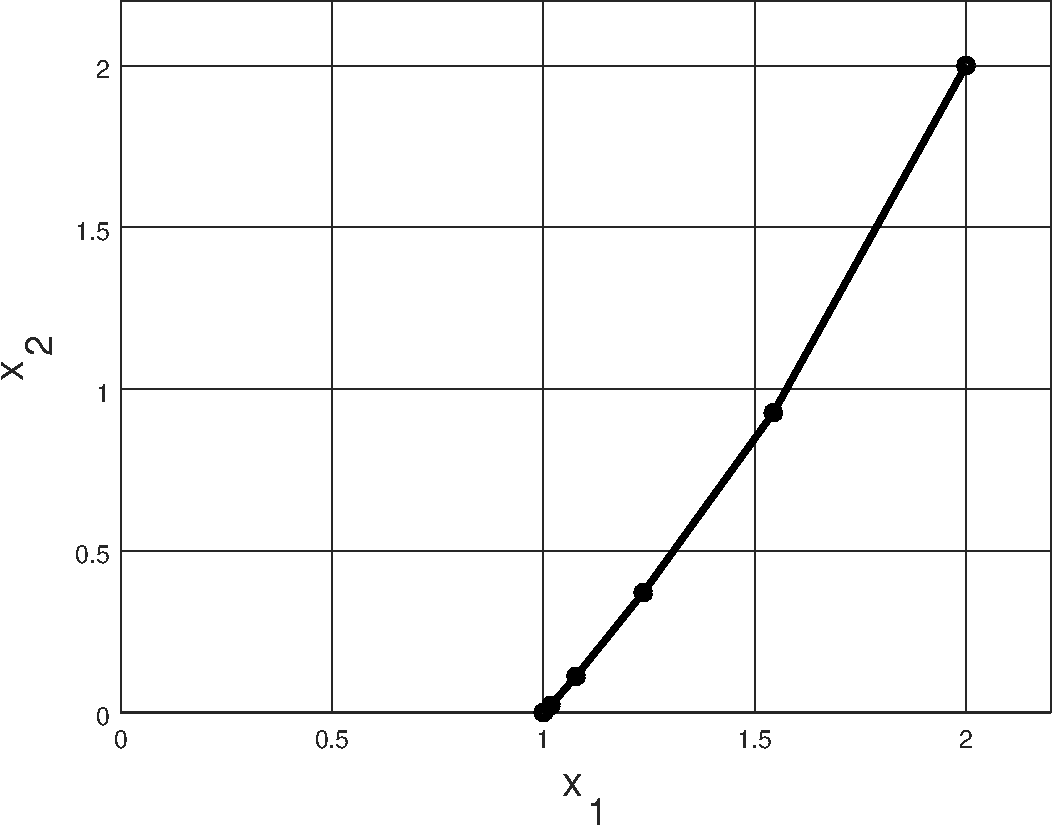
\includegraphics[width=0.6\textwidth]{testpopdip}
\end{center}


\subsection*{Possible improvements}

We may consider possible improvements of our algorithm.  First, in Algorithm 16.1 the computation of the Newton search direction is followed by separate line searches in $x$ and in $\lambda$.  These line searches only maintain nonnegativity and they do not seek sufficient decrease of $f(x)$; they only use ratio tests.  Secondly, equation \eqref{newtonstep} can be symmetrized by multiplying the second half of the equations by $-\Lambda^{-1}$:
\begin{equation}
\begin{bmatrix}
\grad^2 f(x) & - I \\
-I & - \Lambda^{-1} X
\end{bmatrix}
\begin{bmatrix}
\Delta x \\
\Delta \lambda
\end{bmatrix}
=
\begin{bmatrix}
-\grad f(x) + \lambda \\
x - \mu_k \Lambda^{-1} e
\end{bmatrix}
 \label{symmnewtonstep}
\end{equation}
These facts suggests two possible changes:
\begin{enumerate}
\item Back-tracking line search is appropriate as a globalization even for unconstrained optimization.  Thus there must be cases where it is appropriate for problem \eqref{minproblem} as well.  Once the ratio tests are applied, further back-tracking could be used based on sufficient decrease.  Compare the modified back-tracking line searches in \cite{BensonMunson2006}.
\item One can replace linear system \eqref{newtonstep} with symmetrized system \eqref{symmnewtonstep}.
\end{enumerate}
Determining if these are actual improvements would require testing which we have not done.


%\subsection*{Application to example problem (\texttt{glacier}).}
%FIXME a primal-dual interior point method for a glacier problem appears in \cite{Calvoetal2003}

\medskip

\bibliography{doc}
\bibliographystyle{siam}

\end{document}

